\documentclass[main.tex]{subfiles}

\begin{document}

\section{Monitoring System}
\label{section: monitoring}
\textit{This section will go over the solution for a monitoring system for the \gls{psu}. The chapter will tackle the characteristics of the system and what is needed for this project, along with the choice of time-series database used to store the data points. Features such as the specification of storing monitoring data and displaying it to the user using third party software will also be discussed. Finally, it will go over different types of data filtering and how Panda data frame can be used to customize the filtering of data points }

\subsection{Overview}

 The microcontroller on the \gls{mb} directly controls and monitors the current, temperature and voltage usage of the strings and most importantly is responsible for turning off the strings if any of these threshold values are exceeded. The microcontroller is responsible for turning off the strings due to it being a time-critical event, any delay in turning off the strings can lead to damaging the chips. There is however still a need for the user to know what is happening on the \gls{mb}. Knowing what the current draw is, and temperature of the strings is important to be able to effectively troubleshoot the \gls{dtc} while performing runs. It is therefore necessary to create a monitoring system from client-side that can retrieve the monitoring data from the \gls{mb} and display it to the user. It is logical to store the data in a time series database, and the data points from the database can be displayed using third-party software. Not all data retrieved is valuable to the user, data points that only differ between the last point by a margin less than the uncertainty of the measurement is meaningless to track. The data points should therefore be down-sampled in some way to reduce data storage and strain on the database server.

 InfluxDB is chosen as monitoring database due to it being a popular time series database and its compatibility with the graphing tool Grafana, which allows us to display the data with professional graphing tools. Influx and Grafana also features intuitive web interfaces that is highly customizable and easy to work with. Influx also supports the Telegraf plugin, which allows for seamless monitoring of database performance. 
 
 Timing of the client side monitoring is also important, even though there is no time critical operations from the client. The user should be able to quickly assess the status of the \gls{mb} with little delay to more accurately be able to diagnose any faults during a run.
 
 \autoref{fig: pcs_monitoring} shows the overview of the \gls{pcs} and highlights the monitoring system, along with its respective database.
 
 \begin{figure}[!htpb]
    \centering
    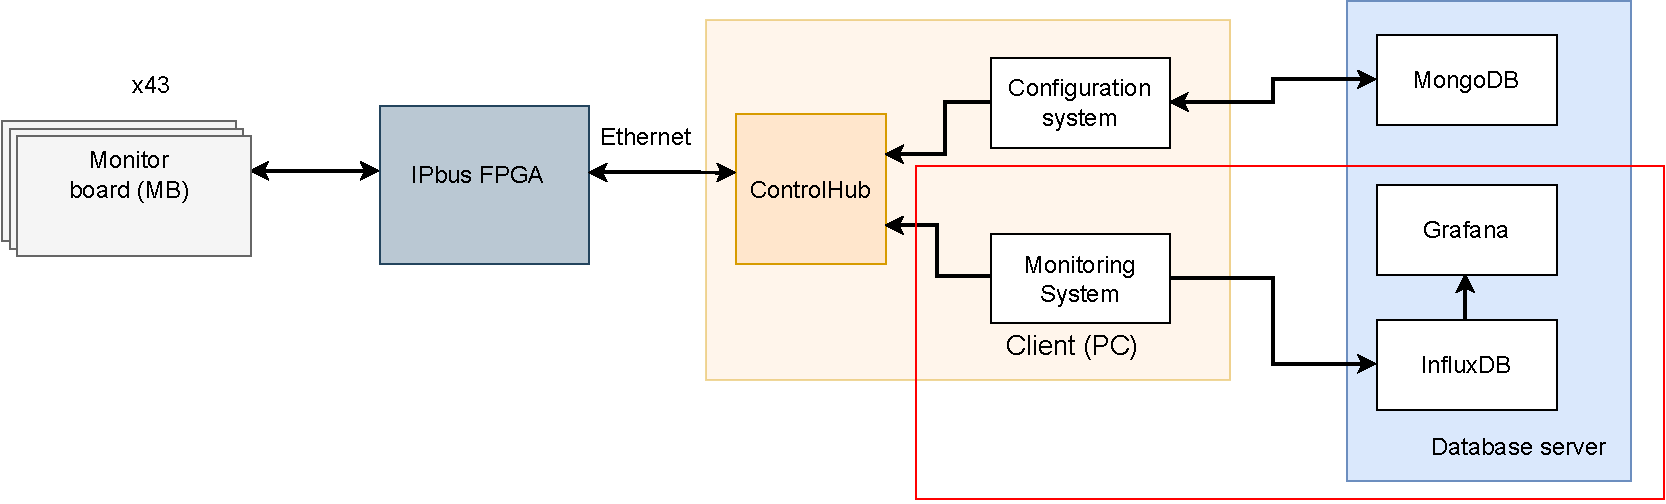
\includegraphics[width=17cm, scale=1.5]{images/PCS overview_monitor.pdf}
    \caption{PCS overview, highlighting the monitoring system.}
    \label{fig: pcs_monitoring}
\end{figure}
\FloatBarrier
 
 The monitoring system sends data to InfluxDB and Grafana interfaces with InfluxDB to display the data points. 

\notinmain{subsections eg bør ha med: monitoring API, InfluxDB, Grafana, Filtering/pandaframe, characteristics of monitoring operation}


\subsection{Monitoring API}
The monitoring system shown in \autoref{fig: pcs_monitoring} is made of several classes that is responsible for retrieving data from the \gls{mb}s, process it, and send it to the database. A dedicated monitoring \gls{api} class is created for the system, which handles data polling and interfaces with the database. A class diagram of the monitoring \gls{api} hierarchy is shown in \autoref{fig: monitor_hierarchy}.

 \begin{figure}[!htpb]
    \centering
    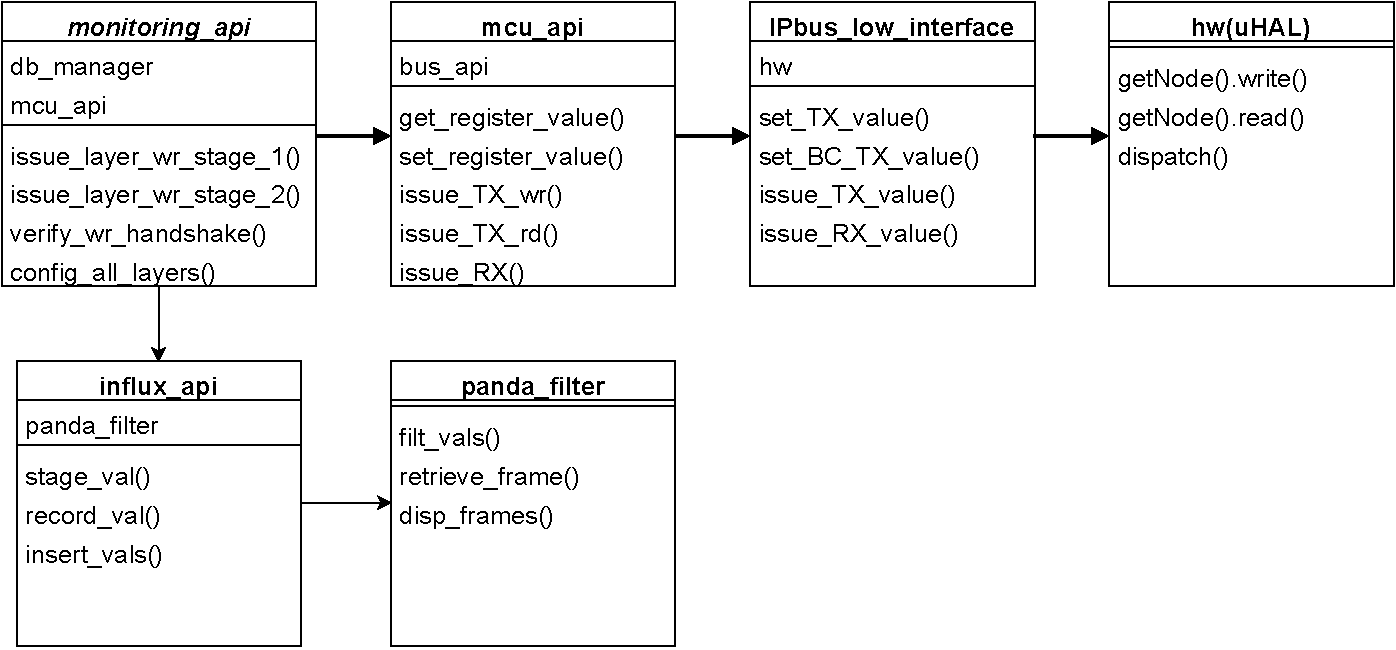
\includegraphics[width=17cm, scale=1.5]{images/monitor_interface_hierarchy.pdf}
    \caption{Interface hierarchy for the monitoring system.}
    \label{fig: monitor_hierarchy}
\end{figure}
\FloatBarrier

The top level of the \gls{api} interfaces with the microcontroller through the \textit{mcu\_api}. The database is interfaced using a custom class, \textit{influx\_api}, which interfaces with the influx API to store data in the database and also filter the data using pandaframe custom class. The main function of the monitoring API class is to poll the data from the microcontroller and insert it into the influx database. 

Polling the data involves retrieving the measured voltage and current of DVDD, AVDD and PWELL, as well as retrieving the measured temperature reading from the PT100 element. In addition to this, the monitoring API must be able to handle errors from the \gls{mb}. The microcontroller have an error count, and an error message register, the error count counts the number of errors that have occurred during the run, and each byte in the message register contains a corresponding error code. The monitoring API must also poll these registers during the monitoring, which requires its own process. \autoref{fig: monitor_flow} shows the flowchart performed when the polling function is called.

\begin{figure}[!ht]
    \centering
    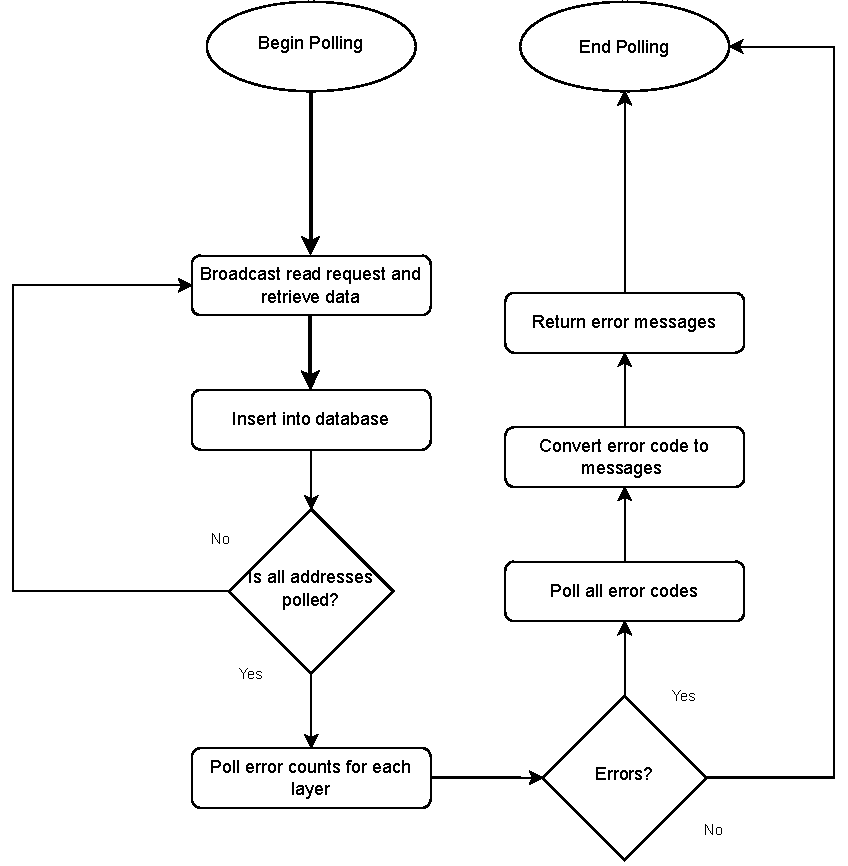
\includegraphics[scale=0.9]{images/Monitoring Flowchart.pdf}
    \caption{Flowchart of the polling operation performed during the monitoring process.}
    \label{fig: monitor_flow}
\end{figure}
\FloatBarrier

The polling the data is relatively simple, it uses the microcontroller API to broadcast and retrieve the data from all of the monitoring addresses. The error handling is a bit more complex, it polls the error count register of each layer and if there are errors, it will retrieve all error codes from the error code register. The error codes are then converted to messages and the function returns a nested list containing error message info from each layer so that it can be relayed to the logging database. Important to note The polling function is only performed once when called, the interface using the API is responsible for looping it continuously during a monitoring operation. The errors are also returned so that the GUI can display it for the user while the monitoring process is running.

The monitoring \gls{api} polls data based on the name tuples stored in the \textit{monitor\_addr} list in the \textit{mcu\_addr} package. This means that one can freely change the monitoring addresses by adding or removing tuples in the list. This is useful if changes to the monitoring process are made, and also makes it easier to repurpose the \gls{api} to other control systems in the \gls{pct}-project. In addition, each error message has a corresponding named tuple which is used to convert error code to message, as well as indicating the severity of the error. This information is used when inserting the messages into the logging database.

\notinmain{Skriv mer her når eg har faktisk laget denne klassen, pluss gui osv. nevn og g options her}

\subsection{Monitoring GUI}

The actual monitoring and overseeing of the polled data is done by Grafana which is discussed in \autoref{ssec: grafana}, but we still need a user interface for starting the monitoring process, as well as booting up the Grafana web application. For this purpose, a custom \gls{gui} for the monitoring system is designed using PyQt5 in the same manner as the configuration \gls{gui} discussed in \autoref{ssec: cgui}. An image of the monitoring \gls{gui} is shown in \autoref{fig: monitor_gui}

\begin{figure}[!ht]
    \centering
    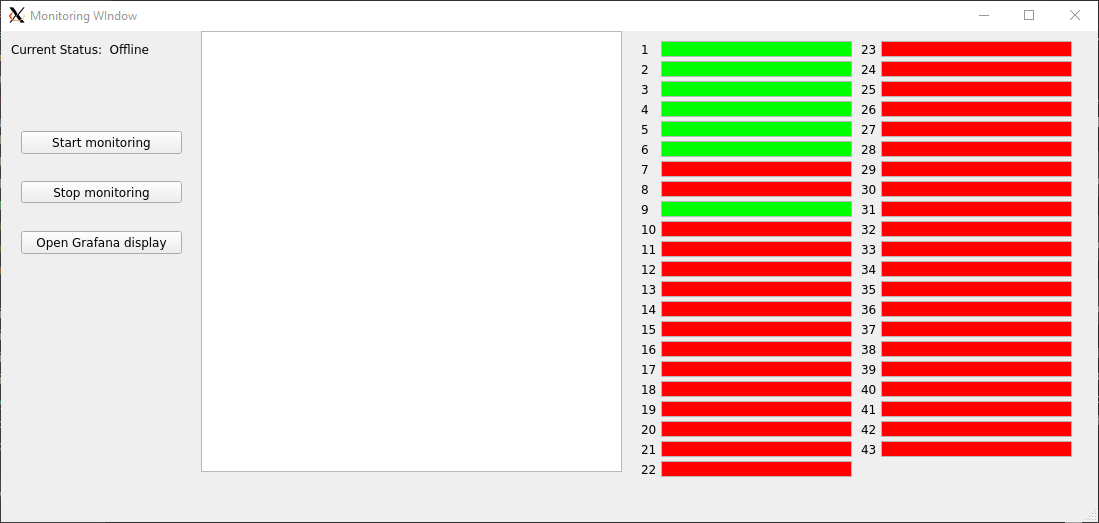
\includegraphics[scale=0.6]{images/monitoring_gui.png}
    \caption{Image of the monitoring GUI, showing the buttons for managing the polling, as well as the log window.}
    \label{fig: monitor_gui}
\end{figure}
\FloatBarrier

The \gls{gui} is relatively simple, having buttons for starting and stopping the monitoring, as well as one for opening the grafana display in the web browser. The log window notifies the user when the monitor process begins, as well as displaying any errors from the monitoring directly. These errors are also sent to the database. It also graphically displays which layers are active on the right side, where green is on and red is off. Note that this pattern only notifies if a com\_module is turned off on the \gls{fpga}, not the actual layers themselves.

\subsection{InfluxDB}
\label{ssec: influxdb}
Monitoring the data from the \gls{mb} requires a database to store these values. A time series database stores data points along with a time stamp, allowing for plotting the data points as a function of time. There are many time series databases available on the market and they come with their own benefits. It was chosen to use InfluxDB for this project. InfluxDB is a popular, open-source, time series database featuring many plugins and APIs that can be integrated with the database. Among these plugins is Grafana, another popular web tool, used for visualizing data and plotting graphs with professional, easy to use interfaces. InfluxDB also features a web interface that can create query requests without knowing the syntax.

The InfluxDB web interface has a graphing tool, where queries can be set up and data can be displayed in various manners, such as graphs or histograms. An image of the tool is displayed in \autoref{fig: influx_explore}

\begin{figure}[!htpb]
    \centering
    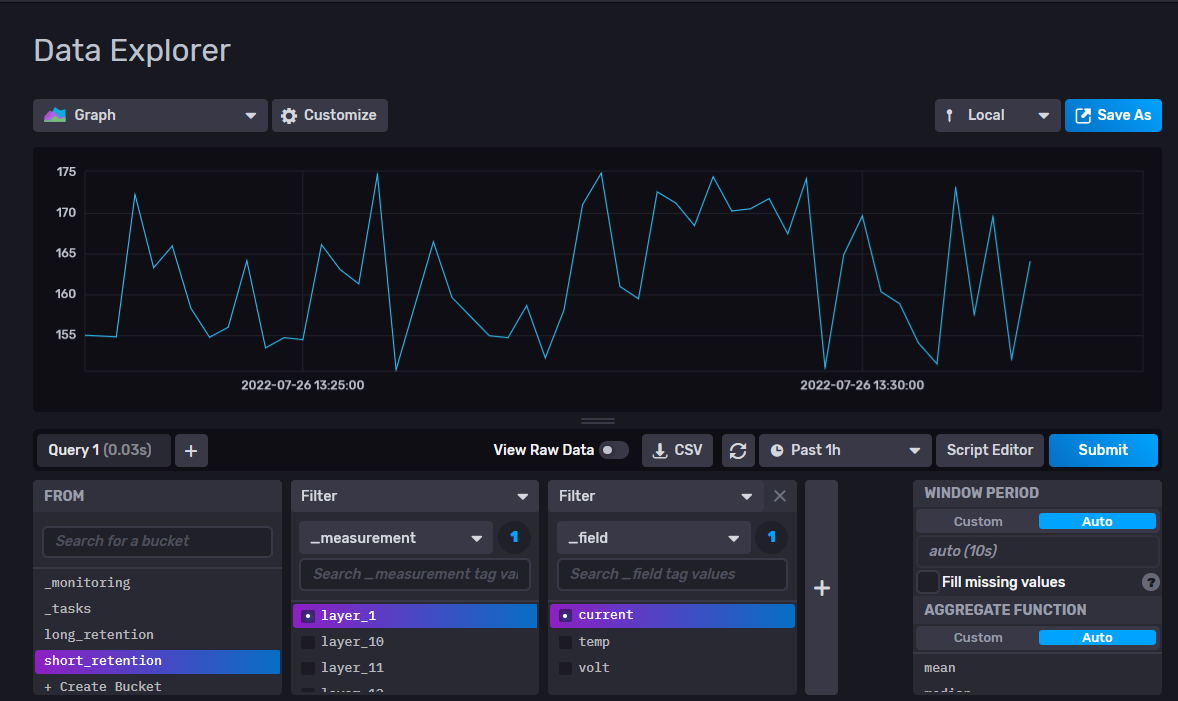
\includegraphics[width=17cm, scale=4]{images/influx_explore.png}
    \caption{Image of the explore tab in the influx web interface.}
    \label{fig: influx_explore}
\end{figure}
\FloatBarrier

The explore tab is useful for observing the data and viewing the raw data as it is inserted into the database. The lower part of \autoref{fig: influx_explore} shows the query tabs, which can be used to create queries from your buckets. The web interface also allows for creating dashboards, where many individual graphs can be displayed at once, the Telegraf plugin, which is mentioned later this section, is made of such a dashboard.

InfluxDB V2 is used for this project, the main difference between previous versions and V2 is the use of the new functional data scripting language specifically designed for InfluxDB, called Flux. Flux is designed to unify querying and processing data in the database, able to retrieve the data points from the database and automatically filter them. This query language is integrated into the web interfaces for both InfluxDB and Grafana, both having example queries that can be generated without needing to know the syntax of Flux. An example of a Flux query is shown in \autoref{fig: flux_example}.

\begin{figure}[!htpb]
    \centering
    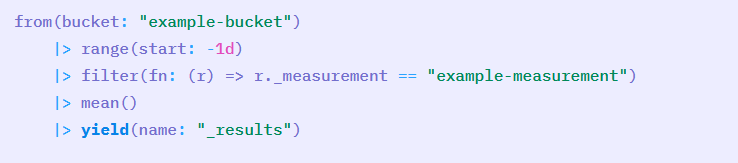
\includegraphics[width=17cm, scale=4]{images/flux_example.png}
    \caption{Example of a flux query retrieving data and filtering it.}
    \label{fig: flux_example}
\end{figure}
\FloatBarrier

In the example, the "\textit{from}" command chooses which source the data should be retrieved from, "\textit{range}" specifies the time range to be filtered and "\textit{filter}" can filter the data based on tags, or measurement type. The "\textit{mean}" function calculates the average of the values, Flux has many functions for filtering the data points based on common filtering techniques. Example of filtering options supported in InfluxDB is calculating mean, nth point filter, median, only unique values, or derivative of the data points.


The setup of the database must also be considered, how many buckets to use, their retention policy and filtering options. All of this can be defined and modified in the InfluxDB web interface. Storing large amounts of data points for long periods of time is often resource heavy and unnecessary, it is therefore logical to store the data points in a bucket with a short retention policy. For longer periods of time, the data can be filtered and sent to a different bucket with longer retention policy. InfluxDB supports this type of operation internally using Flux querying. 

The filter performed on the data points should reduce the amount of points, while also minimizing the amount of information lost. Filtering the data points will be discussed in section blablabla\notinmain{pandaframe filtering subsection}.

InfluxDB also supports the Telegraf plugin, which allows for quick and easy monitoring of the database performance. This is useful for obtaining metrics on the database while the monitoring is performed. \autoref{fig: telegraf_example} shows the Telegraf plugin window in the web interface.

\begin{figure}[!htpb]
    \centering
    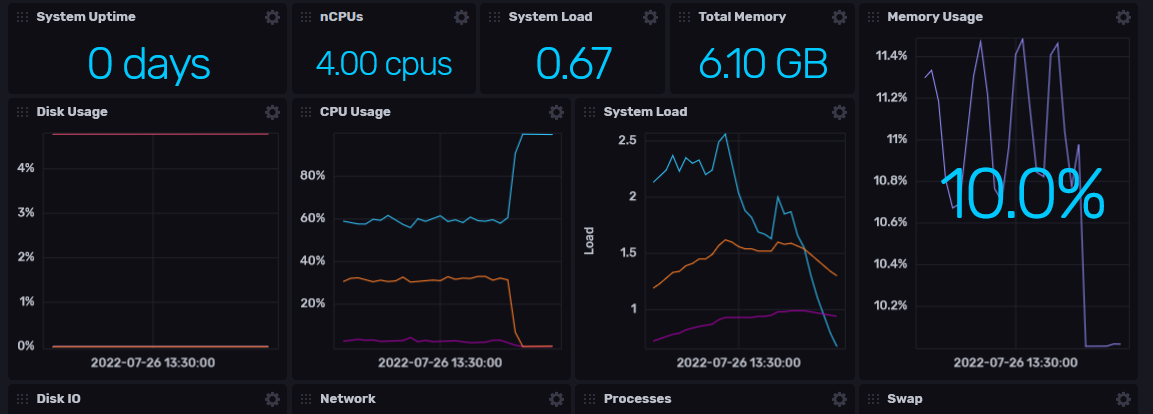
\includegraphics[width=17cm, scale=4]{images/telegraf_example.png}
    \caption{Image of Telegraf plugin displaying various metrics of the database.}
    \label{fig: telegraf_example}
\end{figure}
\FloatBarrier

Telegraf is used to measure the impact the monitoring operation has on the database. This will be discussed more in \autoref{ssec: char_mon}.

\subsection{Grafana}
\label{ssec: grafana}
Grafana is an open source, interactive web interface that can display data in a magnitude of ways. It can provide graphs, histograms, chart solutions for displaying your data in a web application. Grafana was chosen as the graphing tool for this project due to its ability to display data in a clear, concise manner, its ability to create interactive plots and is directly compatible with InfluxDB.

Grafana is hosted on a server, but unlike InfluxDB and MongoDB, we do not need to create our own API communicate with it. Connecting Grafana to influxDB and setting up the dashboard for the monitoring can all be performed in the Grafana web interface. After connecting the Influx database to Grafana, setting up graphs for Grafana to plot is as simple as setting up a Flux query for the specified measurement.

For this project, we want a dashboard that is clear, shows off all the measurements being retrieved from the \gls{mb}s, making it easy for the user to spot abnormalities such as high temperature quickly. There are three different measurement types and 43 layers for each measurement that needs to displayed. Plotting 43*3 graphs on a single dashboard would lead to much clutter on the screen. The solution for this is to instead plot a histogram of each measurement, showing the last recorded value in the database. Grafana's interactive plots lets us set a hyperlink in each histogram that points to the Grafana graph of the respective histogram's measurement. This gives the user an overview of all measurements and the ability to quickly assess each measurement individually with one click.

an overview dashboard was created in Grafana and an image of this dashboard is shown in \autoref{fig: grafana overview}.

\begin{figure}[!htpb]
    \centering
    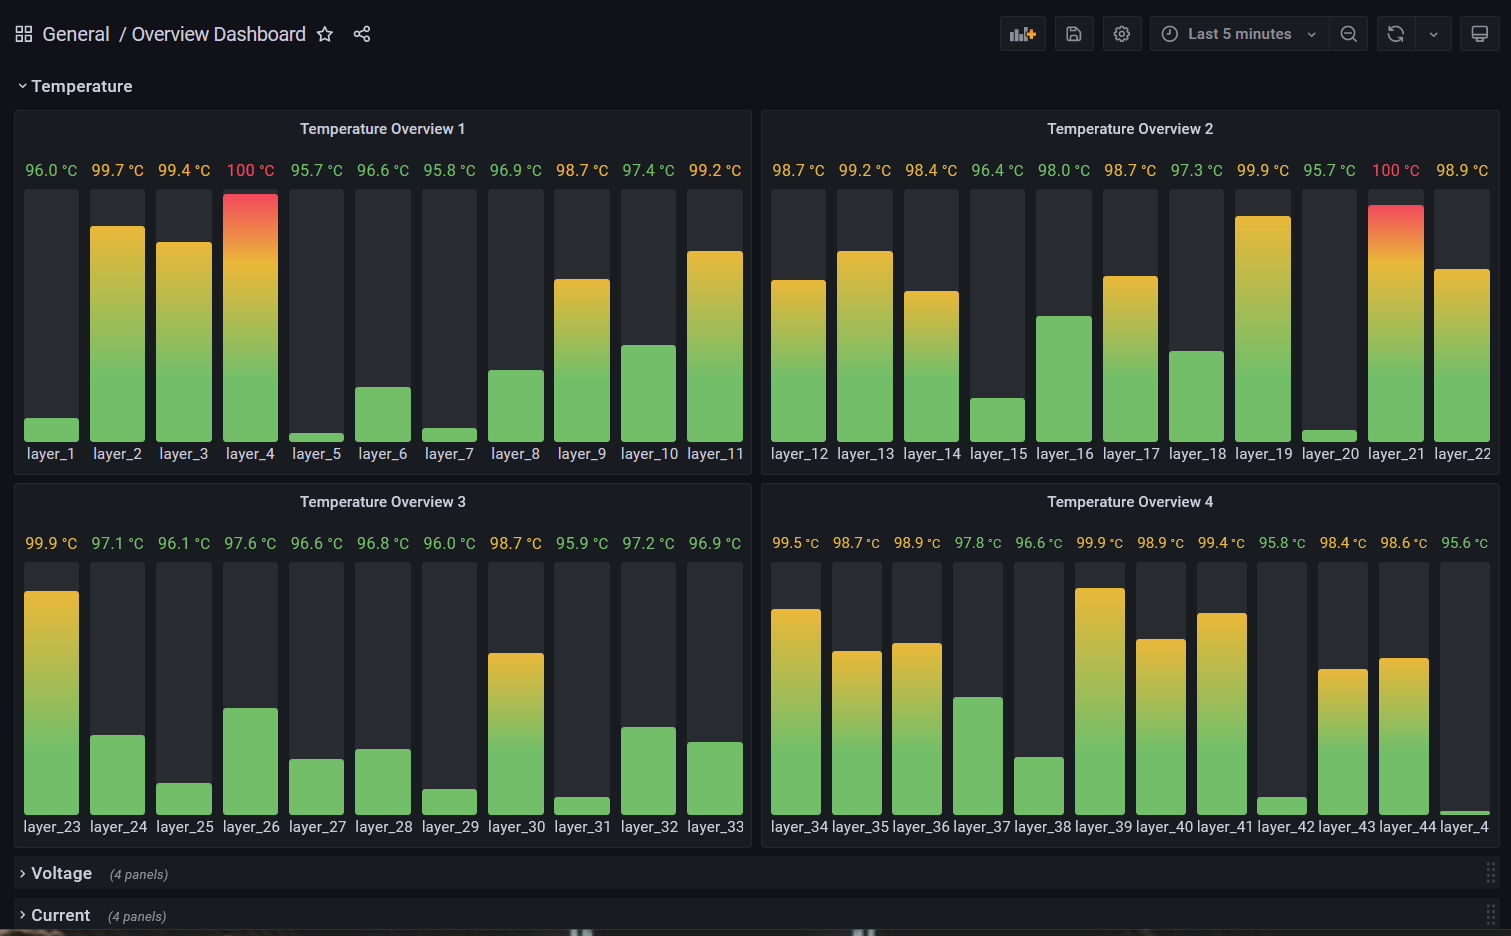
\includegraphics[width=17cm, scale=4]{images/grafana_overview.png}
    \caption{Image of the overview dashboard inside the Grafana web application.}
    \label{fig: grafana overview}
\end{figure}
\FloatBarrier

The above figure shows the overview dashboard displaying arbitrary data that has been inserted into the Influx database. The dashboard is made out of three rows, one for each measurement type, and clicking on a histogram will lead to a second dashboard that plots the data as a function of time for the measurement the user clicked on. The second dashboard is made of three plots, one for each measurement type. A custom variable is added to this dashboard that allows the user to change the layer from which the measurements are retrieved from. An image of the second dashboard is shown in \autoref{fig: grafana second}.

\begin{figure}[!htpb]
    \centering
    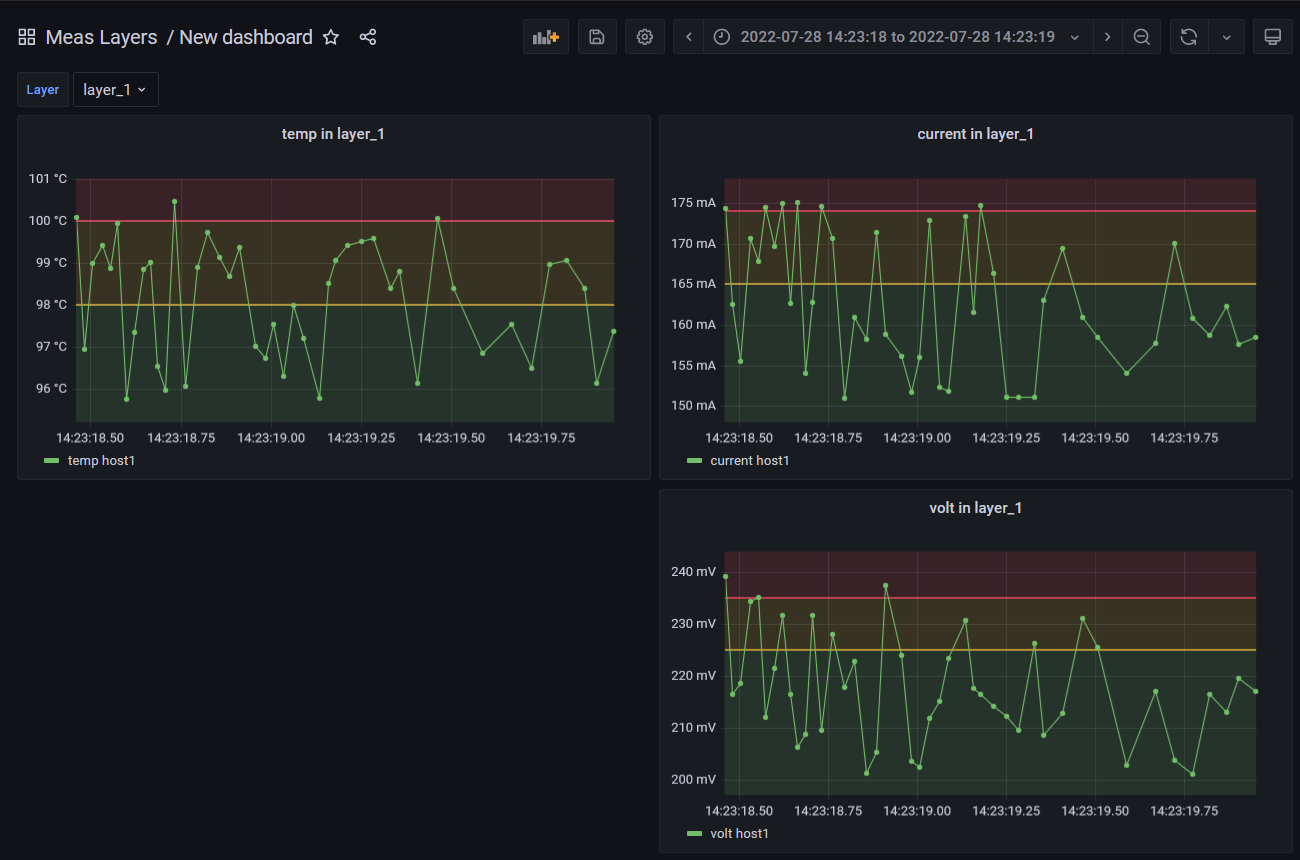
\includegraphics[width=15cm, scale=4]{images/grafana_2nd_dashboard.png}
    \caption{Image of the measurement dashboard inside the Grafana web application.}
    \label{fig: grafana second}
\end{figure}
\FloatBarrier

Using these two dashboards allow for easy and seamless monitoring of the data retrieved from the \gls{mb}s. Both dashboards are exported to JSON-format and stored on the GitHub repository. Setting up the dashboards on a new Grafana server would only require uploading the JSON-document for each dashboard onto the Grafana web application. Lastly, it is worth mentioning Grafana uses Flux queries to retrieve the data, meaning filtering options using Grafana directly is possible.

Although it is worth mentioning that the overview graphic display comes with a fault, the user can only see one type of measurement at once in a window. If it is of value to see two measurement types at once, for example DVDD and temperature, the user would have to either copy the dashboard onto a new window, or they would have to scroll between the two. Grafana contains many tools that may allow us to condense all the info to fit one screen, but there was not enough time while working to perform this re-design.

\notinmain{snakke om flux, vise eksempel, og så kanskje oppsettet av databasen, retention policy}

\subsection{Characteristics of monitoring operation}
\label{ssec: char_mon}
The specifications of the monitoring system is vital to know when designing it. aspects as read and write speeds, storage space and database performance are all important characteristics that needs to be determined before we can begin designing and assess the system.

\notinmain{del denne opp i subsubsections}
\subsubsection{transmission speed of PCS}
During the monitoring operation, current, voltage and temperature must be read for all 43 layers, along with the error register. This leads to reading 4*43 registers every time we poll the \gls{mb}s. There is no inherent reason to have a delay between the polling, so polling the data as often as possible is the logical step to take. The transmission speed of the data will then not only determine the speed of data acquisition, but also the amount of data points received per second, which determines how much storage space is needed, and the sampling rate of the measurements.

\autoref{ssec: con_timing} shows the calculating of the transmission speed from client software to microcontroller, \autoref{eqn:write_delay_equation} shows that a single transmission will take approximately 288 microseconds. For the monitoring system, a read request must be sent to all layers and then client software must retrieve the data from the RX register of every com\_module. This translates to writing to the global TX register and reading 43 registers from the com\_modules. This action must be performed 4 times, to get all measurements. The time for polling all measurements from every layer once then becomes:

\begin{equation} \label{eqn:monitoring_timing}
4*(t_{write}+t_{\mu } + 43*t_{read}) = 4*(250\mu s + 33 \mu s + 43*250\mu s) = 44132 \mu s = 44.132 ms
\end{equation}

The read speed of IPbus is assumed to be 250 microseconds in this calculation. We can now assume that one poll of all measurements will approximately take 44 milliseconds. The amount of data points retrieved per second will then be:

\begin{equation} \label{eqn:data_points_per_second}
\frac{1}{0.044132}*4*43 =  22.659 * 4*43 \approx 3897
\end{equation}

The monitoring system polls all measurements approximately 23 times every second, which leads to retrieving approximately 3897 data points every second. The sampling rate is then 23 times per second, which is acceptable for our use.

Furthermore, a test was performed to measure the timing of polling the data. This test used the prototype setup of the \gls{pcs} mentioned in \autoref{ssec: test_setup}. The main limitation of this test is that the test setup only has one layer connected to the \gls{fpga}, meaning we can only poll one layer during the test. We should therefore expect that the measured polling time to be shorter than the calculated one. if we use \autoref{eqn:monitoring_timing} to calculate the speed of polling one layer, then the timing is found to be 2.132 ms.

The test will poll all data points once and record the time spent polling them, it will then repeat this process 1000 times and find the average of the data. The results, along with comparison of the calculated values is shown in \autoref{tab:monitor_speed}.

\begin{table}[h]
\centering
\begin{tabular}{||c c c||} 
 \hline
  Calculated timing(43 layers) & Calculated timing(1 layer) & Measured timing(1 layer) \\ [0.5ex] 
 \hline\hline
    44.132ms & 2.132ms & 8.7ms ($\sigma$ = 3.4ms) \\  [1ex] 
 \hline
\end{tabular}
\caption{\label{tab:monitor_speed} Comparison of the polling timing of the monitoring API}
\end{table}
\FloatBarrier

The polling timing for polling a single layer was also calculated. Polling the test setup took 8.7 ms with a standard deviation of 3.4 ms. Comparing the calculated timing of polling one layer with the measured timing, we can see that the measured speed fits well with the calculations. the discrepancy between the two values can be explained by the time measurement method not being completely accurate to the data transfer. 

\subsubsection{Storage Space}
Storage space is a vital part of the database, and is determined by many factors. The storage space needed for this project is determined by the amount of data retrieved every second, the resolution of said data, the retention policy of the buckets in the database and how much space is needed to store the data points in the database.

The amount of data retrieved every second has already been calculated in \autoref{eqn:data_points_per_second}, amounting to 3897 data points per second. The type of data stored in the monitoring operation, excluding any log messages, is float numbers. The resolution of the float numbers is the amount of decimal points used for the data point, and therefore this must be decided beforehand. The temperature will not change erratically, an accuracy up to the first decimal point is therefore acceptable. The current and voltage is measured in mA and mV, respectively, already giving us a high level of precision. The voltage is measured by a shunt capacitor that can read voltages up to 250 mV and temperatures will obviously not exceed 1000 degrees, so 4 decimals is a reasonable resolution to store the data in, giving us one decimal point accuracy for both current and temperature. This translates to needing 3 bytes, or 12 bits to store the information in our database. In the InfluxDB hardware sizing guidelines, it is stated that a non-string value requires approximately 3 bytes of data to be stored. Note that this guideline is specified for Influx V1, but we can safely assume this also applies for Influx V2. This leads us to requiring 6 bytes of storage for a single data point. The amount of bytes of data stored each second will then be: 

\begin{equation} \label{eqn:total_bytes_per_second}
3897*4 = 15588 
\end{equation}

Which becomes 16 about kilobytes per second. Lastly, the retention policy of the database determines the max amount of storage space needed. The long retention database is set to have a retention of 30 days, giving us:

\begin{equation} \label{eqn:total_bytes_total}
15588*60*60*24*30 = 40.4 * 10^9
\end{equation}

In total for the long retention database, a storage space of 40.4 gigabytes is required. This is a relative small amount of storage space required and filtering of the data points can lead to reducing the space requirement even more. By applying the same formula from \autoref{eqn:total_bytes_total} for the short retention database, with a retention of 24 hours, the storage space will only amount to 1.34 gigabytes. In total, storage for the monitoring database amounts to 41.74 gigabytes.

\notinmain{Gjør ein test run av databasen og sjå hvor mye plass den tar og sammenlign med kalkulert verdi}


\subsubsection{Optimizing data acquisition}

InfluxDB comes with a variety of options to optimize the data acquisition process. These different options can have a significant impact on the data acquisition and must be considered to ensure it is a good fit for our system.

InfluxDB features several write options for its Python client: Synchronous, Asynchronous and Batching writes. The default option used is batching writes, which is what is considered optimal for InfluxDB. Batching writes collects a specified amount of data points and when full, establishes a https connection with the database and sends the data. This process is very quick in comparison to synchronous writes, which has to establish a https connection for every data point.

The batching size can be customized by the user, but the optimal batch size for influxDB is 5000\cite{influx_batching}. The drawback of the batching is that data will not be sent until the batch is full. A large batching size can lead to long wait times until the data is sent to the database, but this is not a problem if we keep a batch size 5000. The database would get updated about every second in this instance.

We can compare the speed of different batching sizes by inserting a specified amount of data points into the database and record the time taken. \autoref{tab:specs} shows off the time difference between 5, 50, 500, 5000, 50 000 batch size.

\begin{table}[h]
\centering
\begin{tabular}{||c c c||} 
 \hline
 N/A & N/A & N/A \\ [0.5ex] 
 \hline\hline
 Write speed & 38.2s & 5.1s \\ 
 \hline
 System Load & 7 & 78  \\
 \hline
 mean CPU Usage & 545 & 778 \\
 \hline
 4 & 545 & 18744\\
 \hline
 5 & 88 & 788\\ [1ex] 
 \hline

\end{tabular}
\caption{\label{tab:specs} INCOMPLETE}
\end{table}
\FloatBarrier


 
 
 \subsection{Downsampling of InfluxDB}
 


 Downsampling is the process of removing sample points in a signal and it is crucial to do for three reasons: first, to save disk space used for storing the data, second, to reduce network traffic, and last, to increase performance of your server. Recording data from a sensor inadvertently leads to redundant data points. If the measurement remains static over a greater period of time, recording high resolution data of essentially the same value is a waste of space. Additionally, the data is received from an instrument with an uncertainty to its measurements, meaning that storing data points that are within the uncertainty range of the previous data point is also redundant. We want to downsample our data in such a way that we remove as much data as possible, while keeping the information retained.
 
 There are many ways to down-sample your data, there is entire separate fields on the subject, but for this project there is no need to downsample with cutting edge technology. However, efforts should still be made to avoid storing too much redundant data. It is important for this monitoring system to record abnormal data points, i.e. spikes in the measurement data, which can help us diagnose issues with the \gls{dtc}. Therefore using mean or similar filters, results in too coarse of a filtering to be used in this project(this does not mean that these filters should never be used, but they are not suitable for a short retention database).
 
 Creating a custom filter that fits our system is one solution, the question then becomes what type of filter fits the best. A filtering technique used by OSIsoft in their PI servers seems promising to base our own filter on, due to it focusing on filtering data from instruments. The technique uses what is know as an exception and compression rule, that aims to reduce the amount of data points from an instrument while retaining the information of the graph. The exception filter is based on removing data that can be perceived as noise from the sensors. \autoref{fig: osisoft_exception} shows how this is implemented in OSIsoft's PI servers.
 
\begin{figure}[!htpb]
    \centering
    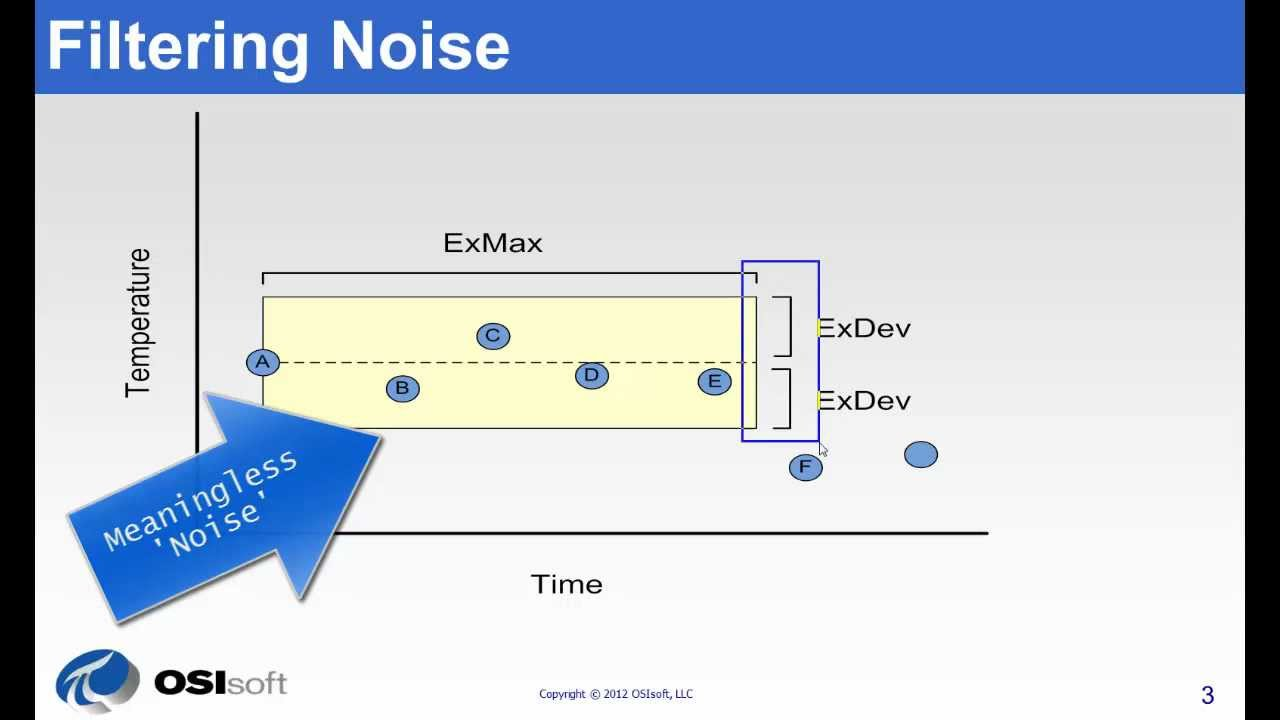
\includegraphics[width=15cm, scale=4]{images/osisoft_exception.jpg}
    \caption{Image showcasing an example the exception filter. Points in the deadband is dropped by the filter\cite{osisoft_exception}}
    \label{fig: osisoft_exception}
\end{figure}
\FloatBarrier 
 
The filter starts with a "snapshot" value, point A in the figure, and sets two restrictions on the next points which is defined by the two parameters "ExMax" and "ExDev". "ExDev" defines the deadband of the filter, all points that appear in the deadband is considered noise and are removed from the set. If a point is recorded outside the deadband, then that point becomes the new "snapshot" value that defines a new deadband around it. The "ExMax" attribute determines the time span allowed between two points. If no new values exceeding the deadband is recorded for an "ExMax" amount of time, then the next data point is kept and set to be the new "snapshot" value, regardless if it was in the deadband of the previous snapshot. This is done to prevent too large gaps between recorded data points. Lastly, when a data point exceed the deadband, the previous point will be retained, in the case of \autoref{fig: osisoft_exception}, point E passes the filter because point F exceeded the deadband. This is done to retain the shape of the graph, \autoref{fig: osisoft_last_point} shows a slide from OSIsoft's summary of exception and demonstrates how not retaining the last point can affect the graph.

\begin{figure}[!htpb]
    \centering
    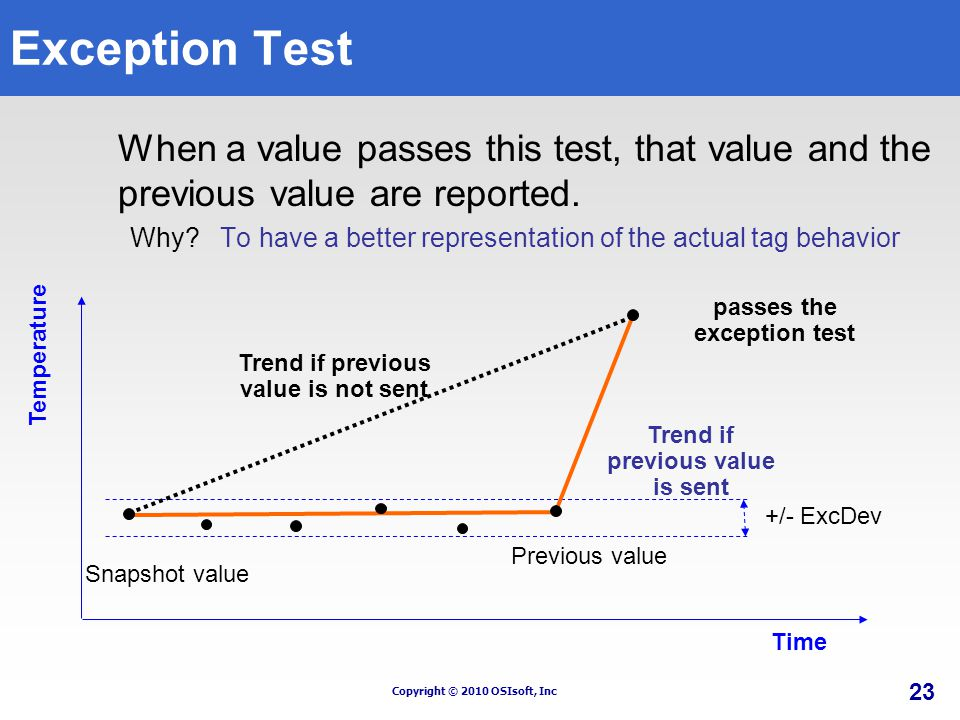
\includegraphics[width=12cm, scale=4]{images/osisoft_last_point.jpg}
    \caption{Slide showing the projected graph depending on if we retain the last point before the snapshot value or not\cite{osisoft_exception}}
    \label{fig: osisoft_last_point}
\end{figure}
\FloatBarrier 
 
 As seen from the figure, the data will be misinterpreted if we do not consider the data point before the new snapshot value. 
 
 Lastly we can mention the compression technique which uses a "swinging door" algorithm to remove redundant data points. The process makes a line between two points and remove the next data points who's angle in relation to this line is not above a certain threshold. This process is more complicated to implement than the exception test and it is currently seen as unnecessary for this project. The compression test can be revisited in the future if database performance becomes an issue.
 
 Implementing custom filters for our data points means that we must be able to manipulate the data points in a clear fashion before sending them to the Influx database. Pandas dataframe is a two dimensional data structure with rows and axes for efficiently setting up tables of data and manipulating it. InfluxDB is also compatible with Panda dataframes and can be inserted directly into the database. By inserting the data into Panda dataframe, we can analyze the data and modify it as we wish, this allows us to efficiently create custom filters in Python. A custom class, \textit{panda\_filter}, is responsible for managing the pandas dataframes and contain functions to format the inserted data. The class contains three pandaframes, one for each measurement type, the measurements are separated so that the data points can be modified without affecting the other measurement types. The dataframe consists of a column containing the actual data, and a column for the timestamp. \autoref{fig: panda_example} shows an example of the structure of the panda dataframes. 
 
 \begin{figure}[!htpb]
    \centering
    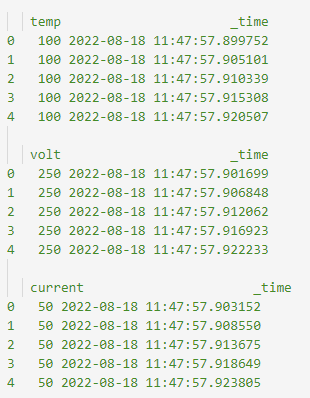
\includegraphics[width=5cm, scale=1]{images/panda_frame_example.png}
    \caption{Image showing the setup of the three dataframes used in the panda filter class.}
    \label{fig: panda_example}
\end{figure}
\FloatBarrier 

The index is the leftmost value, followed by the measurement type column and lastly the timestamp column, which uses the "timedate" library format. The InfluxDB client supports panda dataframe, but the index must be set to the timestamp for it to be accepted by the client. The panda filter class automatically set the timestamp to be the index when outputting the dataframes.

Another layer of downsampling is performed between the short retention and the long retention buckets in InfluxDB. The long retention bucket stores data for historical purposes and high resolution data is not needed, therefore a mean, or nth sample filter can be performed between the two buckets. The data flow for the monitor system is shown in \autoref{fig: data_process}.

 \begin{figure}[!htpb]
    \centering
    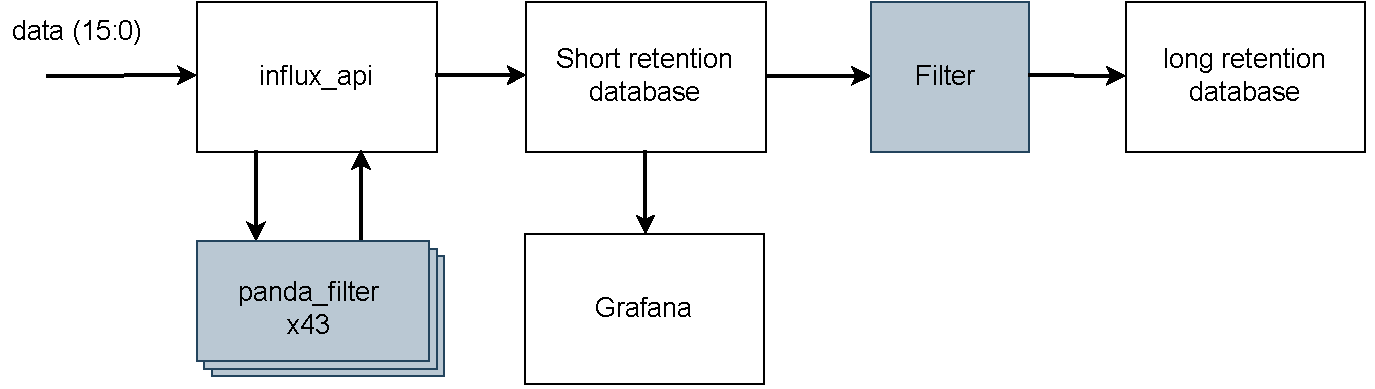
\includegraphics[width=18cm, scale=1]{images/processing data overview.pdf}
    \caption{Block diagram of data being processed through the monitoring system.}
    \label{fig: data_process}
\end{figure}
\FloatBarrier 

The \textit{influx\_api} class instantiates 43 \textit{panda\_filter} objects that stores the data points and gives them a timestamp. When \textit{influx\_api} sends the data to the database, it retrieves the dataframes from the \textit{panda\_filter} and sends it to the short retention database. All data sent to the short retention database is also sent to Grafana to be displayed, additionally, the data is filtered and inserted into the long retention database. The filter between the short and long retention is by default a mean filter, but it can be changed easily by editing the flux query of the long retention database.

 

 






\end{document}